\section{Обзор существующих решений}
\label{sec:Section2} \index{Section2}

\subsection{Формат сигнатур}

Прежде чем говорить непосредственно о методах автоматической генерации сигнатур, стоит сначала понять,
какие бывают сигнатуры и в каком формате они могут быть представлены.

Существует несколько представлений сигнатур. Некоторые из этих видов использовались для представлений сигнатур червей.
В работе \cite{newsome2005polygraph} приводится следующая классификация:

\begin{itemize}
    \item \textbf{Конъюнктивная сигнатура}: состоит из набора подстрок (или токенов).
    Полезная нагрузка соответствует ей, если все токены в наборе были найдены в любом порядке.
    \item \textbf{Сигнатура, представленная последовательностью токенов}: состоит из упорядоченного набора токенов.
    Полезная нагрузка соответствует сигнатуре, если она содержит всю последовательность токенов в том же порядке.
    \item \textbf{Байесовская сигнатура}: состоит из набора токенов, каждый из которых связан с оценкой, и общего порогового значения.
    Байесовские сигнатуры обеспечивают вероятностное сопоставление: вычисляется вероятность сопоставления,
    используя оценки присутствующих токенов в полезной нагрузки.
    Если результирующая вероятность превышает пороговое значение, то считается, что полезная нагрузка совпала с сигнатурой.
\end{itemize}

При использовании любого из этих определений в качестве определения сигнатуры приложения/протокола возникают
некоторые специфические проблемы:

\begin{enumerate}
    \item \textbf{Разнообразие потоков}: в рамках одного приложения/протокола могут использоваться множество потоков,
    имеющие разные общие подстроки. Например, приложения P2P используют разные протоколы для обмена одноранговой информацией и данными.
    Кроме того приложения будут обновлять свои протоколы.
    Потоки различных версий протоколов могут существовать в сети одновременно.
    Ни сигнатура, представленная токен-последовательностью,
    ни конъюнктивная сигнатура не могут выражать несколько наборов общих подстрок.
    \item \textbf{Взаимоисключающее свойство некоторых подстрок в прикладных протоколах}.
    Например, протокол Gnutella имеет две последовательности подстрок $\{$'Get' 'UserAgent'$\}$ и $\{$'HTTP' 'User-Agent'$\}$.
    Подстроки 'Get' и 'HTTP' не будут отображаться в одном и том же потоке в протоколе Gnutella.
    Две общие подстроки являются взаимоисключающими, но байесовские сигнатуры не могут выражать взаимоисключающее свойство.
\end{enumerate}

Определение сигнатуры, основанное на регулярных выражениях, становится очень распространённым в классификации приложений
\cite{szabo2012automatic, wang2012generating, vinothgeorge2013efficient}.
Однако процесс сопоставления регулярных выражений требует огромной вычислительной мощности,
которая слабо масштабируется для идентификации сетевого трафика в режиме реального времени.
Способ построения регулярного выражения оказывает непосредственное влияние на классификацию потоков
и на общую производительность сопоставления.
Несмотря на это, некоторые системы DPI используют регулярные выражения для представления сигнатур приложений.
Система обнаружения/предотвращения вторжений Snort (IDS/IPS) \cite{Snort}
имеет множество сигнатур приложений и предлагает пользователю возможность вставлять новые регулярные выражения по требованию.

Почти неизвестно алгоритмов извлечения сигнатур в виде регулярных выражений, а те что есть -
основаны на строках и небольшом подмножестве операций регулярных выражений.
Поэтому дальше будем рассматривать сигнатуры только в виде строк.

Среди возможных описаний строковых сигнатур, набор последовательностей подстрок является наилучшим определением сигнатуры.
Полезная нагрузка соответствует сигнатуре, если она содержит какую-то последовательность подстрок из этого набора.
Такое определение решает описанные выше проблемы.

Введем следующее определение: уровень поддержки последовательности подстрок (support) равен отношению количества хостов,
использующих соответствующее приложение или протокол и трафик которого содержит эту последовательность подстрок
к общему количеству хостов, использующих соответствующее приложение или протокол.

При заданном формате, в общем случае, не любая последовательность подстрок из набора охватывает все хосты.
В части из дальнейших рассматриваемых методов считается, что сигнатура состоит из одной последовательности подстрок,
уровень поддержки которой равен 1, то есть она присутствует в трафике каждого хоста, использующего рассматриваемый протокол
или приложение. Этот показатель можно использовать как параметр в некоторых методах.

\subsection{Структура сигнатур}

Большинство форматов сигнатур в предыдущих работах \cite{park2008towards,ye2009autosig,santosautomatic}
представляют собой простые подстроки, которые часто появляются в полезной нагрузке.
Следовательно, всё ещё существует вероятность того, что извлеченные сигнатуры полезной нагрузки могут быть не специфичными
для конкретного протокола, некоторые могут принадлежать и другому протоколу. Это называется избыточностью сигнатур.

Для улучшения качества сигнатур предлагается выделить три типа сигнатур \cite{goo2016payload, shim2019automatic}:

\begin{enumerate}
    \item сигнатура содержимого (полезной нагрузки),
    \item сигнатура пакета,
    \item сигнатура потока.
\end{enumerate}

Сигнатура содержимого определяется как различимая и уникальная подстрока полезной нагрузки, состоящая из непрерывных символов или
шестнадцатеричных значений. Очень трудно обеспечить уникальность с помощью одной подстроки. Например,
такие строки <<GET>>  или <<HTTP>>, которые часто встречаются в HTTP, не могут служить конечными сигнатурами,
так как они не различают приложения.

Сигнатура пакета состоит из серии сигнатур содержимого, которые появляются в одном пакете.
Так как классификация может выполняться без накопления пакетов, то есть без сбора потока, то анализируется всегда хотя бы один пакет.
Это значит, что для классификации всегда можно использовать сигнатуры пакетов, и не имеет смысла использовать отдельно сигнатуры
содержимого.

Сигнатура потока состоит из серии сигнатур пакетов, которые появляются в одном потоке, где под потоком понимается набор пакетов,
имеющий одни и те же IP-адрес источника, IP-адрес назначения, порт источника, порт назначения и
используемый протокол транспортного уровня. Сигнатура потока гораздо более специфична для конкретного приложения,
чем сигнатура пакета, и значительно повышает точность.

Поэтапный процесс извлечения сигнатур представлен на рис. \ref{signature_process}.
Данная структура сигнатур обладает свойством вложенности.

\begin{figure}[H]
    \begin{center}
        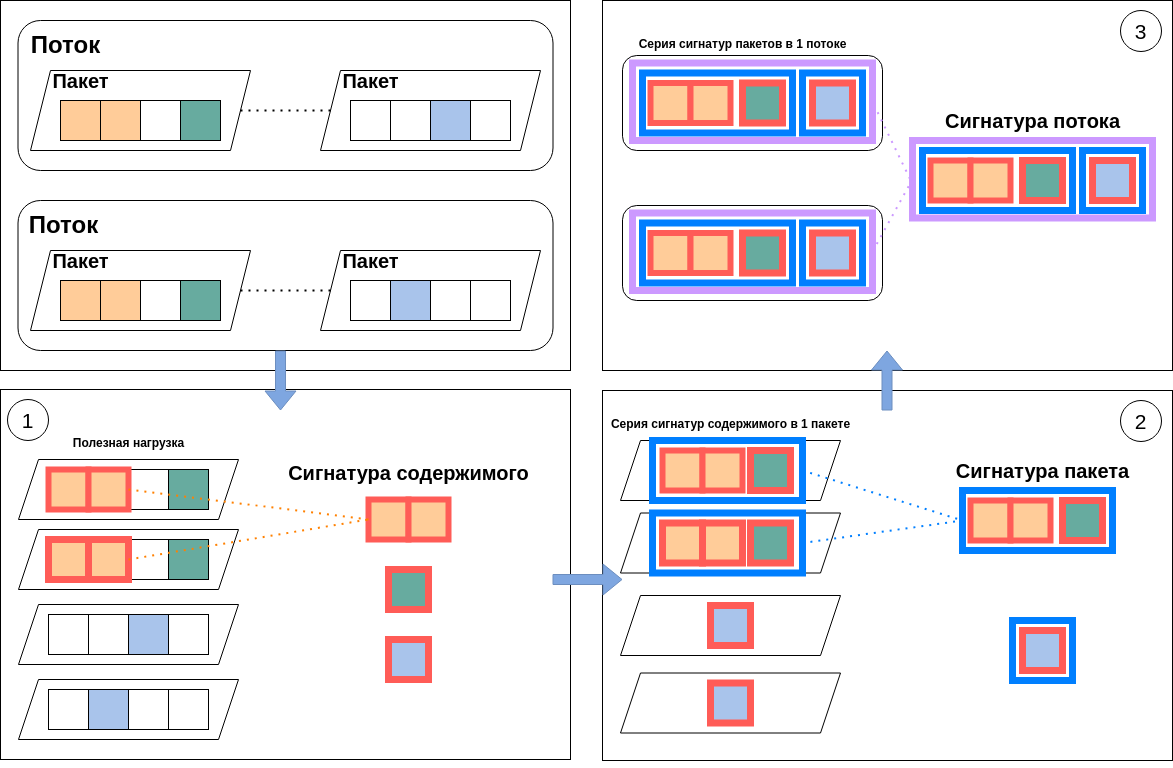
\includegraphics[width = \textwidth]{signature_structure.png}
        \caption{Процесс извлечения предлагаемой структуры сигнатур полезной нагрузки.}\label{signature_process}
    \end{center}
\end{figure}

\subsection{Метрики оценки качества сигнатур}

Для оценки качества получаемых сигнатур будем рассматривать результаты мультиклассового классификатора.
Выходом такого классификатора будет служить набор классов, сигнатурам которых соответствует полезная нагрузка потока.
В реальности классификатор следует останавливать при первом соответствии сигнатуре,
но в рамках исследований будет проверяться на соответствие каждой сигнатуре каждого класса.

Рассмотрим матрицу ошибок для мультиклассовой классификации. Так как все последующие показатели удобно рассчитывать
для случая бинарной классификации, то на рис. \ref{ConfusionMatrix} показан переход от мультиклассовой к бинарной классификации.

\begin{figure}[h!]
    \begin{center}
        \includesvg[width = 0.5\textwidth]{multiclassification.svg}
        \caption{Матрица ошибок в мультиклассовом случае. Переход от мультиклассовой классификации к бинарной.} \label{ConfusionMatrix}
    \end{center}
\end{figure}

Для неё вводят следующие четыре категории, к котором можно отнести результат работы классификатора на полученной сигнатуре:

\begin{itemize}
    \item истинно положительный (TP): указывает, что поток правильно классифицирован, как относящийся к определенному классу.
    \item истинно отрицательный (TN): указывает, что поток правильно классифицирован, как не относящийся к определенному классу.
    \item ложно положительный (FP): указывает, что поток неправильно классифицирован, как относящийся к определенному классу.
    \item ложный отрицательный (FN): указывает, что поток неправильно классифицирован, как не относящийся к определенному классу.
\end{itemize}

Наиболее часто используемые показатели для классификации трафика определяются следующим образом:

\begin{itemize}
    \item Accuracy (достоверность) - доля правильных классификаций.
    $$ accuracy = \dfrac{TP + TN}{TP + TN + FP + FN} $$

    \item Recall (полнота) - отношение верно классифицированных потоков определенного класса к общему числу потоков этого класса,
    то есть описывает способность сигнатуры обнаружить данный целевой протокол или приложение.
    $$ recall = \dfrac{TP}{TP + FN} $$

    \item Precision (точность) - доля верно классифицированных потоков среди всех потоков, которые классификатор отнёс к этому классу.
    $$ precision = \cfrac{TP}{TP + FP} $$

    \item $F_1$-score ($F_1$-мера) - гармоническое среднее между точностью и полнотой.
     $$ \textit{$F_1$-score} = \dfrac{2 \times recall \times precision}{recall + precision} $$
    Метрика accuracy может терять свой смысл в задачах с сильно неравными классами.
    Напротив же recall и precision не зависят от соотношения классов и поэтому применимы в случае несбалансированных классов,
    что является верным для сетевого трафика. Часто на практике возникает задача найти оптимальный баланс между precision
    и recall. Для этих целей подходит F-мера, которая достигает максимума при recall
    и precision равным 1, и стремится к минимуму, если хотя бы один из параметров стремится к нулю.

\end{itemize}

Для сигнатур полезно ещё ввести такое понятие как:

\begin{itemize}
    \item Redundancy (избыточность) определяется как:
    $$ \textit{Redundancy} = \frac{\text{Число потоков, идентифицированные двумя и более сигнатурами}}{\text{Число потоков, идентифицированные набором сигнатур}}$$
    Redundancy имеет значение от 0 до 1, где 0 - наилучшее значение, которое указывает на то, что все сигнатуры набора классифицируют исключительно только свою часть трафика,
    то есть являются уникальными и незаменяемыми. Если redundancy близка к 1, то в наборе присутствует ненужные сигнатуры, которые идентифицируют перекрывающийся трафик.
    По мере увеличения количества сигнатур увеличиваются и накладные расходы системы, поэтому данное значение должно оставаться низким.
\end{itemize}

\subsection{Обзор существующих методов автоматической генерации сигнатур}

Рассмотрим несколько существующих методов автоматической генерации сигнатур и опишем основной принцип их работы.

\subsubsection{LASER}

В статье \cite{park2008towards} описан алгоритм LASER (Application Signature ExtRaction),
который основан на задаче поиска наиболее длинной общей подпоследовательности LCS (Longest common subsequence).
Данный алгоритм автоматически определяет достоверный шаблон в полезной нагрузке пакета без предварительного знания форматов протоколов, то есть генерирует сигнатуру пакета.
За шаг извлечения сигнатуры был принят алгоритм LCS, который ранее в основном использовался для сопоставления последовательностей ДНК в приложениях биоинформатики \cite{ning2006finding}.
Он был модифицирован под текущие задачи.

Вводятся ограничения на модификацию LCS:

\begin{itemize}
    \item \textbf{Количество пакетов в потоке}.
    Нет необходимости проводить проверку над всеми пакетами в наборе,
    потому что сигнатура существует в нескольких начальных пакетах потока.
    \item \textbf{Минимальная длина подстроки}. Стоимость сопоставления сигнатур пропорциональна их длинам.
    Сгенерированная сигнатура состоит из последовательности подстрок.
    Чтобы избежать каких-либо тривиальных сигнатур,
    минимальная граница длины подстроки должна рассматриваться как ограничение для модифицированного алгоритма LCS.
    Имея это ограничение длины, предотвращается включение однопозиционных и многопозиционных символов в последовательность общих строк,
    например символа '/' в HTTP пакетах.
    \item \textbf{Сравнение размера пакетов}. Это увеличивает вероятность нахождения надёжной сигнатуры,
    если пакеты сгруппированы по назначению (например, управляющий трафик или трафик загрузки) и характеристикам трафика.
    Одной из таких характеристик является размер пакета. Объём данных при установлении соединения небольшой.
    Конкретная сигнатура существует только в первых пакетах.
    Поэтому сравнения небольших пакетов установки соединения и пакетов загрузки нежелательно для генерации надёжной сигнатуры.

\end{itemize}

Поясним идею алгоритма. На вход алгоритма подаётся набор потоков, в которых содержится хотя бы по packet\_constraint
(параметр алгоритма) пакетов. Выбираются два потока, для которых происходит полный попарный перебор пакетов,
и если разница размеров пакетов в паре меньше threshold (параметр алгоритма),
то вызывается функция LASER для этой пары пакетов (поиск наиболее длинной общей подпоследовательности).
Выбирается самая длинная общая подпоследовательность среди всех результатов вызовов LASER.
Затем происходит процесс уточнения: проходим по всем оставшимся потокам, вызываем функцию LASER
для всех пакетов из выбранного потока и текущей сигнатуры,
среди результатов выбирается самая длинная общая подпоследовательность.
Когда потоки закончились, возвращаем полученный результат.

Функция LASER представляет собой алгоритм Needleman-Wunsch, в котором используется матрица направлений,
но в результат попадают не все подстроки, а только те, что длиннее min\_substring\_length\_constraint (параметр алгоритма).

Таким образом, у алгоритма LASER 3 параметра настройки:
\begin{itemize}
    \item packet\_constraint (количество пакетов в потоке)
    \item threshold (порог разницы размеров для сравнения пакетов)
    \item min\_substring\_length\_constraint (минимальная длина подстроки)
\end{itemize}

\subsubsection{AutoSig}

Следующий рассматриваемый метод называется AutoSig \cite{ye2009autosig, santosautomatic}.
Каждый поток из выборки обрабатывается как последовательность байт из первых N байт полезной нагрузки.
Данный алгоритм генерирует сигнатуру-потока, являющуюся набором общих последовательностей подстрок.
Приведем описание работы алгоритма.

Сначала алгоритм делит содержимое потоков на небольшие блоки содержимого фиксированного размера, которые называются шинглами.
Чтобы исключить шумы, шинглы делят на разные группы в зависимости от их смещения. Как видно из рис. \ref{autosig:shingles} шинглы разделены на разные окна.
Окна перекрываются и имеют фиксированную ширину 2W. i-е окно покрывает полезную нагрузку, которая расположена от $i \times W$ байта до $(i+2) \times W$ байта,
поэтому размер области перекрытия между двумя окнами равен размеру W. Шингл будет считаться общим, если он встретился в одном и том же окне более, чем в $R \cdot N$ потоках,
где $N$ - количество потоков, $R$ - порог выбора общего шингла.

\begin{figure}[h!]
    \begin{center}
        \includesvg[width = 0.6\textwidth]{autosig.svg}
        \caption{Схема выделение шинглов и окон в алгоритме AutoSig.}\label{autosig:shingles}
    \end{center}
\end{figure}

Затем при помощи адаптивного алгоритма слияния перекрывающиеся общие шинглы объединяются в подстроки.
Для оценки их слияния используется показатель

$$ sim(x, y) = \frac{|flows(xy)|}{|flows(x) \cup flows(y)|} $$

где $flows(x)$ - потоки, содержащие шингл $x$, а $flows(xy)$ - потоки, содержащие шинглы $x$ и $y$ вместе (смежные или перекрывающиеся, иначе $sim(x, y) = 0$).
В алгоритме адаптивного слияния шингл $x$ и шингл $y$ объединяются, если $sim(x, y)>S$, где $S$ - предопределенное пороговое значение.
Наконец, строится дерево подстрок для организации общих подстрок в конечные сигнатуры. Пример такого дерева представлен на рис. \ref{autosig:tree}.

\begin{figure}[H]
    \begin{center}
        \includesvg[width = 0.6\textwidth]{autosig_tree.svg}
        \caption{Дерево подстрок в алгоритме AutoSig.}\label{autosig:tree}
    \end{center}
\end{figure}


Серые узлы являются узлами сигнатуры. Корневой узел дерева подстрок является пустой подстрокой.
Каждый путь от узла сигнатуры к корневому узлу соответствует последовательности подстрок.
Он формируется подстроками в узлах вдоль пути (исключая корневой узел).
Дерево подстрок обладает следующими свойствами:

\begin{itemize}
    \item Каждый узел соответствует общей подстроке и набору потоков F.
    Каждый поток в этом наборе содержит общую подстроку.
    Общая подстрока корневого узла является пустой строкой, будем считать, что она содержится во всех потоках.
    \item если узел P является родительским узлом узла A, набор потоков F(A) является подмножеством набора потоков F(P).
    Это подразумевает, что поток, принадлежащий узлу A, не только содержит общую подстроку узла A, но также содержит общую подстроку своего родительского узла P.
    Например, потоки узла `INFO' содержат подстроки `INFO' и `\$CMD:'.
    \item Если набор потоков узла является строгим надмножеством объединения наборов потоков его дочерних узлов, узел является узлом сигнатуры.
    В противном случае это не узел сигнатуры. Корневой узел не является узлом сигнатуры. Листья являются узлами сигнатуры.
    Например, на рис. \ref{autosig:tree} узел `FAIL' является узлом сигнатуры, а узел `TOUCH' - нет.
    Потоки, содержащие подстроку `TOUCH', также содержат подстроку `FAIL'.
    Вместо двух последовательностей подстрок $\{$`TOUCH', `FAIL'$\}$ и $\{$`TOUCH'$\}$
    генерируется только последовательность подстрок $\{$`TOUCH', `FAIL'$\}$.

\end{itemize}

Построение дерева сигнатур начинается с пустого корня.
Затем общие подстроки сортируются в порядке убывания в соответствии с количеством потоков, в которых они присутствуют.
Потом эти подстроки вставляются в дерево одна за другой.

Для вставки новой подстроки, сначала проверяется является ли набор потоков нового узла подстроки
подмножеством набора потоков текущего узла. Если это верно, то вставка завершается неудачей.
В противном случае пытаемся рекурсивно вставить новый узел подстроки под каждым дочерним узлом текущего узла.
Если все вставки завершатся неудачей, новый узел подстроки будет вставлен как ребенок текущего узла.

Каждый путь от узла сигнатуры к корневому узлу соответствует последовательности подстрок.
Для генерации последовательностей подстрок используется алгоритм поиска в глубину со стеком для записи пути.
После извлечения последовательностей подстрок в дереве каждая последовательность подстрок
переупорядочивается в соответствии со смещением в потоке каждой подстроки.

\subsubsection{SigBox}

Теперь рассмотрим метод, который называется SigBox \cite{shim2017sigbox}. Данный метод основан на алгоритме последовательных шаблонов.
Конечная цель этого алгоритма состоит в том, чтобы найти частые подпоследовательности в наборе входных последовательностей.
Применяется один и тот же алгоритм для извлечения трех типов сигнатур: содержимого, пакета и потока. Изменяется лишь то, какие последовательности
подаются на вход алгоритму и чем является элемент этой последовательности.

В случае извлечения сигнатуры содержимого последовательность содержимого является полезной нагрузкой пакета.
Следовательно, элемент последовательности представляет собой однобайтный символ полезной нагрузки пакета.

В случае извлечения сигнатуры пакета последовательность пакетов представляет собой серию сигнатур содержимого, находящаяся в одной и той же полезной нагрузки пакета.
Следовательно, элемент последовательности пакетов представляет собой индивидуальную сигнатуру содержимого.

В случае извлечения сигнатуры потока последовательность потока представляет собой серию сигнатур пакетов, расположенных в одной и той же полезной нагрузки потока.
Следовательно, элемент последовательности потока представляет собой индивидуальную сигнатуру пакета.

Опишем работу алгоритма последовательных шаблонов.
Сначала извлекаются подпоследовательности длиной 1 из всех последовательностей и сохраняются в наборе подпоследовательностей длиной 1, $L_1$.
Из подпоследовательностей длиной $k-1$ извлекаются все подпоследовательности кандидаты длины $k$,
увеличивая длину до тех пор, пока не будут извлечены все новые подпоследовательности (кандидаты).
Этот итерационный процесс состоит из двух частей.
Сначала из текущего множества исключаются кандидаты, которые не удовлетворяют минимальной поддержке $(1.0)$.
Затем извлекаются кандидаты длиной $k$ с помощью кандидатов длиной $(k-1)$.
В качестве последнего шага проверяется связь включения между подпоследовательностями; если связь найдена, включенные подпоследовательности удаляются.

Чтобы подсчитать уровень поддержки подпоследовательности для заданного множества кандидатов, необходимо сначала найти множество всех хостов для
множества кандидатов, а затем найти множество хостов, последовательность которых содержит заданную подпоследовательность.
Значение поддержки для подпоследовательности равняется отношению мощностей найденных множеств.
В \cite{shim2017sigbox} использовался наивный алгоритм сопоставления, однако авторы советовали заменить на более быстрые алгоритмы
\cite{karp1987efficient,boyer1977fast,xie2010improved,zhou2019research}.

Для извлечения кандидатов длины $k$ используется набор подпоследовательностей длины $k-1$, $L_{k-1}$.
Сравниваются все возможные пары из $L_{k-1}$.
Если $k = 2$, то подпоследовательности в паре объединяются как подпоследовательность длиной 2.
В противном случае, проверяется, что две подпоследовательности перекрываются $k-2$ символами.
В этом случае две подпоследовательности длины $(k-1)$ объединяются, образуя единую подпоследовательность длины $k$.

Предложенная система генерирует сигнатуры содержимого, затем генерирует сигнатуры пакетов и, наконец, генерирует сигнатуры потоков, используя на каждом этапе описанный выше алгоритм.

\newpage
